\chapter{Experimental setup}\label{ch:experimental_setup}

The exerimental setup was largely adopted from Ref.~\cite{Hertlein2017} and we
will only give a brief summary including a short characterization. Amendments
we made include the \gls{rf} signal source of the \gls{aod}.

\section{Optics}

The optical setup can be disected into two parts: a closed first section that
reduces the power of the $\SI{532}{\nano\meter}$ laser source from
$\SI{10}{\watt}$ to below $\SI{2}{\milli\watt}$, it also includes an \gls{aom}
for intensity regulation. The second section is the actual setup where a
\gls{2d} \gls{aod} is used to manipulate the angle of the laser beam in order
to dynamically control the position of the tightly-focused laser beam in the
imaging plane. Both sections are connected through a \gls{smf}.

\subsection{First section: power reduction}\label{subsec:setup_power_reduction}

Because of safety concerns the power reduction section is confined into a
visually sealed box housing. \Cref{fig:setup_power_reduction} reveals the
inside of the power reduction setup.
\begin{figure}[htb]
  \centering
  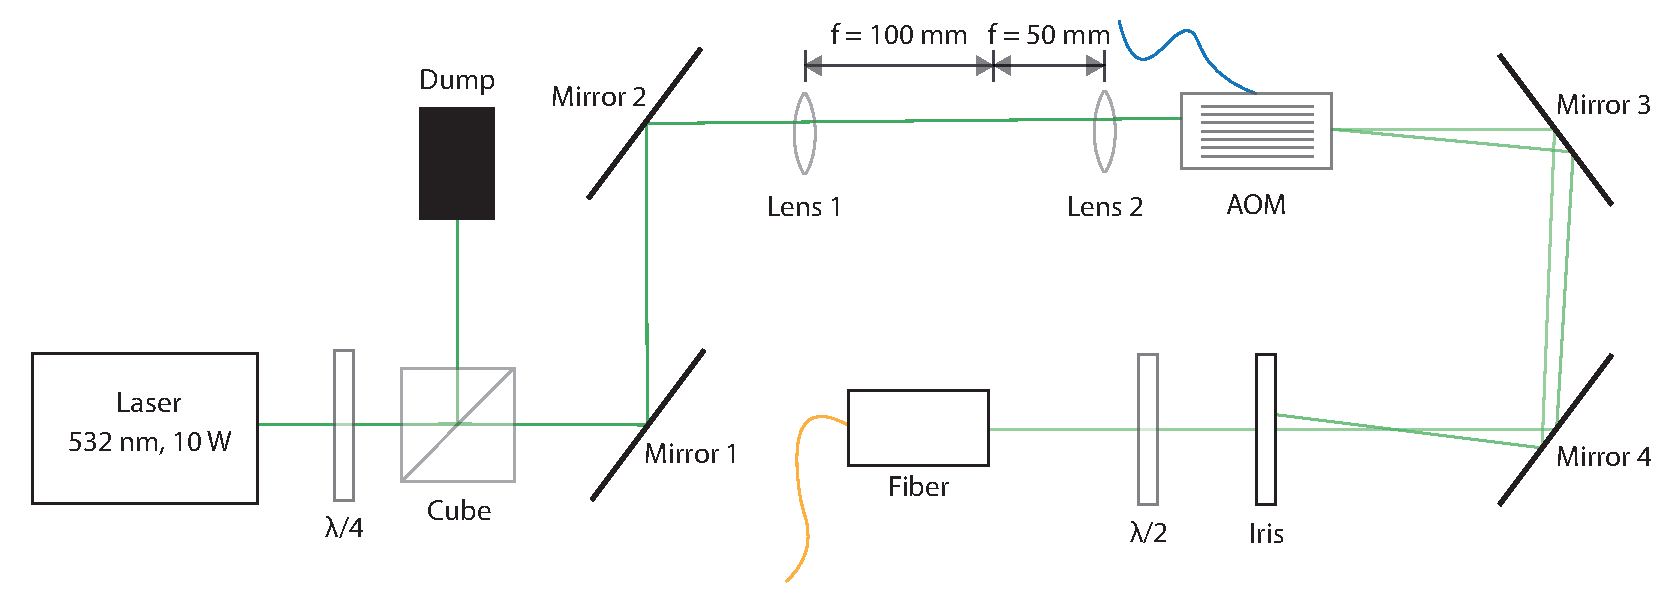
\includegraphics[width=\textwidth]{../figure/setup/power-reduction.pdf}
  \caption{Optical configuration of the power reduction section.
  }\label{fig:setup_power_reduction}
\end{figure}
The laser beam leaving the laser source is linearyly polarized. In order to
divert the majority of the power into a beam dump we use a $\lambda/2$
retarder plate and a high-power polarizing beam splitter. Afterwards Mirror
\num{1} and Mirror \num{2} direct the beam towards the center of a $2:1$
telescope composed of Lens \num{1} and Lens \num{2}. The telescope is there to
reduce the beam diameter by \num{2} in order to avoid cut-off at the aperture
of the subsequent \gls{aom}. The \gls{aom} diffracts the laser beam into
multiple orders as it acts as a tunable diffraction gratting. Mirror \num{3}
and Mirror \num{4} direct theses orders onto a pinhole which is configured to
intromit only the first order deflection. The power in the first diffraction
order can be controlled by changing the \gls{rf} power sent to the \gls{aom}.
Finally a $\lambda/2$ retarder plate is used together with Mirror \num{3} and
Mirror \num{4} to couple the beam with the polarization-maintaining \gls{smf}.

\subsection{Beam deflection and detection}\label{subsec:setup_deflection_detection}

The section for beam deflection and detection as disclosed in
\Cref{fig:setup_beam_deflection} receives the down-powered laser beam from
previously described section by a \gls{smf}. Hereinafter the beam passes a
rotatable retarder plate and beam splitter Cube \num{1} to clean the
polarization of the laser beam after passing through the \gls{smf}. A second
polarizer with Cube \num{2} is used to branch off a part of the beam to
Photodiode \num{1} that is positioned to be at the focal point of Lens
\num{1}. Photodiode \num{1} is connected via a feedback loop with the
amplitude modulation of the \gls{aom} depicted in
\Cref{fig:setup_power_reduction} to stabilize the laser intensity against for
instance thermal drifts.
\begin{figure}[htb]
  \centering
  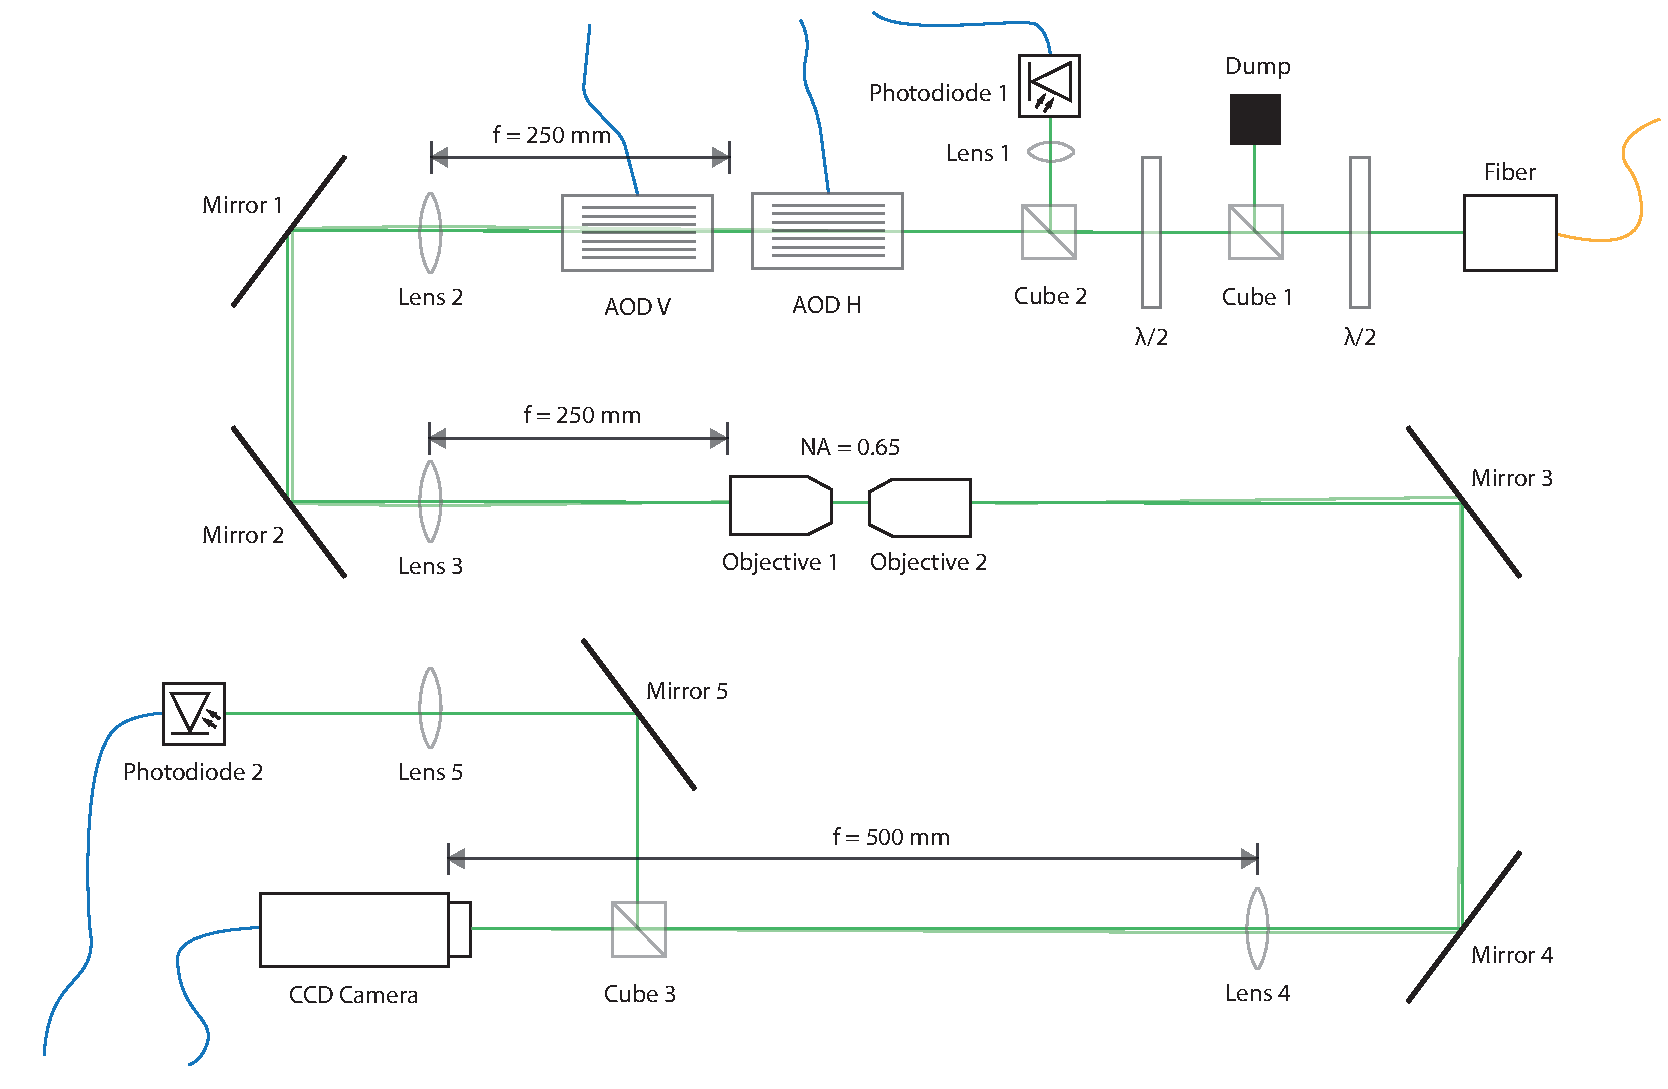
\includegraphics[width=\textwidth]{../figure/setup/beam-deflection.pdf}
  \caption{Optical configuration of the beam deflection section.
  }\label{fig:setup_beam_deflection}
\end{figure}
For horizontal and vertical beam deflection two \gls{aod}s are used. A $1:1$
telescope comprised of two lenses (Lens \num{2} and Lens \num{3}) is used to
image the beam on a pair of objectives. The telescope translates a change in
the incident beam angle to a position offset. The purpose of the first
objective is to focus the laser on to the atom plane. The components described
so far are sufficient to offset a high-resolution pertubation laser
perpendicular to the atomic plane. The purpose of the other components is to
unfocus the laser back for detection. Consecutively the after being unfocused
from the second objective, the laser is reflected by Mirror \num{3} and
Mirror \num{4} to the part intended for detection. Lens \num{4} focuses the
colliminated laser beam on to the camera \gls{ccd} camera sensor. Cube \num{3}
forks a portion of the beam away from the \gls{ccd} camera on o Mirror \num{5}
that guides the beam towards Lens \num{5} in order to focus the beam onto
Photodiode \num{2}. It is important that the sensor of Photodiode \num{2} is
positioned on the focal spot of Lens \num{5}, otherwise the laser beam would
leave the sensor when deflected by the \gls{aod}.

\section{Electronics}

Beforehand we described the optical setups used. Now we want to emphasize
on the electronics and how they are integrated into the optical setup.

In \Cref{fig:setup_elop_aom} the electronic setup of the \gls{aom} control
loop are presented. The \gls{dds} signal source outputs a \SI{80}{\mega\hertz}
\gls{rf} signal which is amplified and then supplied to the \gls{aom} for
intensity modulation. Photodiode \num{1} measures the modulated laser
intensity and is connected to a \gls{pid}. The \gls{pid} outputs a signal
proportional to the deviation of the measured intensity from the configured
intensity which is provided to the amplitude modulation input of the power
amplifier.
\begin{figure}[htbp]
  \centering
  \begin{subfigure}[b]{0.4\textwidth}
    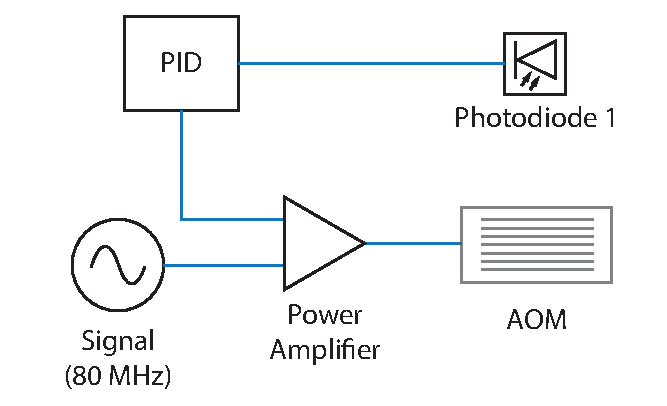
\includegraphics[width=\textwidth]{../figure/setup/aom-control.pdf}
    \caption{Intensity control via \gls{aom}.
    }\label{fig:setup_elop_aom}
  \end{subfigure}
  \begin{subfigure}[b]{0.4\textwidth}
    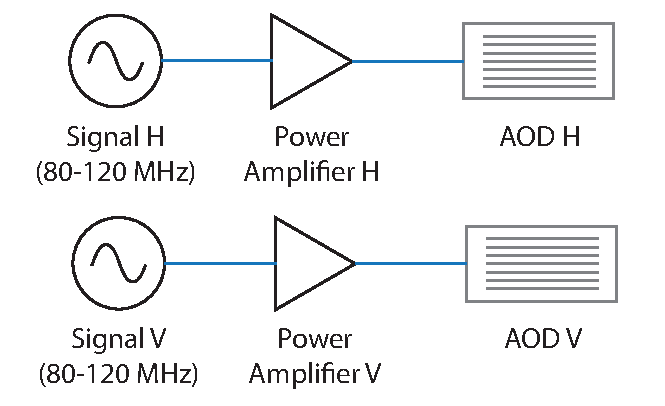
\includegraphics[width=\textwidth]{../figure/setup/aod-control.pdf}
    \caption{Deflection control via \gls{aod}.
    }\label{fig:setup_elop_aod}
  \end{subfigure}
  \caption{Electronic setup used to control the electro-optic devices.
  }\label{fig:setup_elop}
\end{figure}
In \Cref{fig:setup_elop_aod} the electronic setup connecting the \gls{2d}
\gls{aod} with the \gls{dds} signal sources are presented. The \gls{dds}
output is configured through a network interface as we will explain later.
First we will elaborate on the general components used in
\Cref{fig:setup_elop} as well as our experiments.

\subsection{Signal source}\label{subsec:setup_signal_source}

We require the signal source to generate a sinusoidal \gls{rf} signal
\begin{equation}
  x(t)
  =A\cos\left(2\pi ft\right)
  \label{eq:signal},
\end{equation}
where $0\leq A\leq1$ denotes the amplitude and $f$ the frequency. For the
\gls{aom} setup in \Cref{fig:setup_elop_aom} it is sufficient to configure
a constant amplitude $A=1$ and frequency $f=\SI{80}{\mega\hertz}$. For the
\gls{aod} control, however, our requirements are lifted. Ideally we would
like to program a time-dependent amplitude $A(t)$ and frequency $f(t)$,
supplementary to the support of an external trigger signal in order to
syncronize multiple signal sources. For our setup we chose to use \gls{dds}
as signal sources as they provide high frequency resolution, a wide range of
modulation options and are cheap compared to signal generators. In
\cref{ch:digital_signal_synthesis} we will give a more detailed view of the
characteristics and limitations of the \gls{ad9910}, the \gls{dds} \gls{ic}
we use as signal source.

\subsection{Power amplifier}

We use three signal amplifiers with respective input from the signal sources
to have an output power of about $P=\SI{2}{\watt}$ required by the \gls{aod}s
and the \gls{aom} for maximum diffraction efficiency. The used amplifiers
offer a second input for external amplitude modulation. In case of the
\gls{aom} we connect thisinput to the output of the feedback loop.

\subsection{PID controller}

A feedback loop takes a reference $r(t)$, also called setpoint, and a process
variable $y(t)$ as input and outputs the value for a control variable $u(t)$,
which in turn, affects the process that determines $y(t)$. A \gls{pid} is
a specific implementation of such a feedback loop that uses a proportional,
differential and integrative term to estimate the control variable $u(t)$.
\begin{figure}[htb]
  \centering
  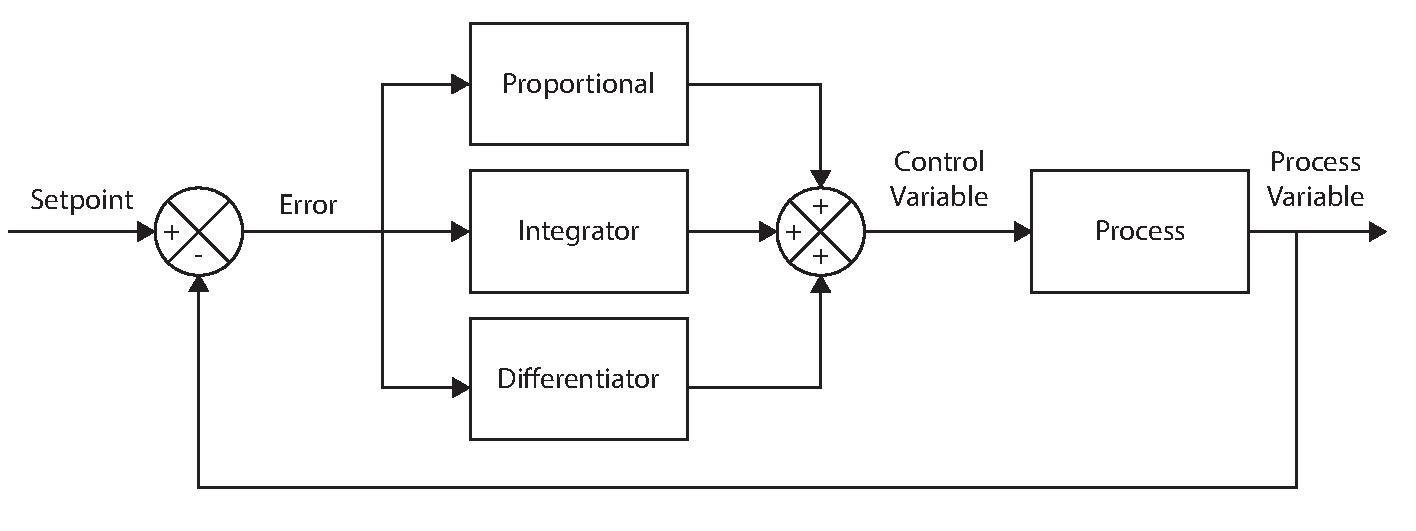
\includegraphics[width=\textwidth]{../figure/setup/pid-controller.pdf}
  \caption{Block diagram of a \gls{pid} feedback loop.
  }\label{fig:setup_pid}
\end{figure}
In \Cref{fig:setup_pid} we see a block diagram of a \gls{pid}. The error
values is supplied to the proportional block as well as the differentiator
and integrator which in sum give the updated control variable value $u(t)$.
The process changes with $u(t)$ and we read off the process variable $y(t)$
we want to regulate and feed it back to the start of the loop. The control
variable of the \gls{pid} can be expressed through
\begin{equation}
  u(t)
  =
  K_p e(t)+
  K_i \int_0^t \dd{t^\prime} e(t^\prime)+
  K_d \dv{t}{e(t)}
  \label{eq:setup_pid},
\end{equation}
where $K_p,K_i,K_d$ denote the coefficients for respective terms. The ideal
values for the coefficients have to be found by loop tunning for each
application. Every term contributing to \cref{eq:setup_pid} can be thought
of to account for a different time scale of the process: the proportional term
considers the momentary error, the differential predicts trends and the
integrator corrects for past errors. For our particular application the
control variable is the amplitude $A(t)$ supplied to the modulation input
of the power amplifier of the \gls{aom} \gls{rf} signal. The process variable
of our \gls{pid} is the voltage measured at Photodiode \num{1}.

\subsection{Trigger source}

To syncronize the signal sources, the \gls{ccd} camera and the oscilloscope
it was necessary to design a network programable trigger source that outputs
a square pulse and forwards it to multiple devices. The schematics, board
layout and source code can be found in the \Cref{app:electronics:trigger_hub}.

\section{Software}

In the last section of this chapter we will see that the diffraction
efficiency of the \gls{aod}s is not constant and requires readjustment by
amplitude modulation of the \gls{rf} signal supplied to the \gls{aod}s. We
consider this readjustment step a calibration process. The efficienct
implementation of such a calibration process requires an orchestrated
interplay of different electronic devices which we will discuss now.

\section{Trial run}

\begin{figure}[htb]
  \centering
  \begin{adjustbox}{width=\textwidth}
    \inputpgf{../figure/intensity/projection/}{bodo.pgf}
  \end{adjustbox}
  \caption{Text projection as captured by the \gls{ccd} camera.
  }\label{fig:setup_projection}
\end{figure}
